% \documentclass[10pt, twocolumn, a4paper]{article}
\documentclass[12pt,a4paper]{article}

\usepackage[backend=biber, style=ieee]{biblatex}                        % To include the bibliography
\usepackage[left=2cm, right=2cm, top=2.5cm, bottom=2.5cm]{geometry}     % To set the margins
\usepackage[noend]{algpseudocode}
\usepackage[table]{xcolor}                                              % For coloring cells

\usepackage{algorithm}                                                  % To include algorithms
\usepackage{amsfonts}                                                   % To include math fonts:ToggleTerm direction=float
\usepackage{amsmath}                                                    % To include Mathematic symbols
\usepackage{authblk}                                                    % To format author affiliations
\usepackage{caption}                                                    % For caption spacing
\usepackage{float}                                                      % To place figures where you want them
\usepackage{graphicx}                                                   % To include images
\usepackage{hyperref}                                                   % To include hyperlinks
\usepackage{lipsum}                                                     % TODO: remove this
\usepackage{listings}                                                   % To include code
\usepackage{tabularx}                                                   % For equal-width columns
\usepackage{tcolorbox}                                                  % To make colored boxes
\usepackage{tikz}                                                       % To draw graphs
\usepackage{titlesec}                                                   % To format section titles
\usepackage{xcolor}                                                     % To define colors

\usetikzlibrary{graphs,graphs.standard}
\usetikzlibrary{positioning}

\addbibresource{./references.bib}

% Esto es para poder hacer cajitas de código con el fondo gris
\lstset{
    language=C++,
    basicstyle=\ttfamily\small,
    keywordstyle=\color{blue}\bfseries,
    stringstyle=\color{green!60!black},
    commentstyle=\color{gray},
    backgroundcolor=\color{gray!05},
    frame=single,
    numbers=left,
    numberstyle=\small,
    stepnumber=1,
    numbersep=10pt,
    tabsize=2,
    showstringspaces=false,
    captionpos=b,
}

% Para poder hacer flechas
\usetikzlibrary{shapes, arrows}

% Sección de definiciones
\titleformat{\section}{\Large\bfseries}{\thesection}{1em}{}
\titleformat{\subsection}{\large\bfseries}{\thesubsection}{1em}{}

% Caja de colores
\definecolor{mint}{RGB}{202,251,202}
\definecolor{yellow}{RGB}{255,255,202}
\definecolor{red}{RGB}{255,202,202}

% Variables globales
\newcommand{\currentsemester}{Segundo Semestre}
\newcommand{\currentyear}{2025}


\begin{document}

\begin{center}
    \LARGE\textbf{Programación Paralela} \\
    \Large{Teórica 01 - Introducción} \\
    \normalsize{Segundo Semestre, 2025} \\
    \vspace{1em}
    \hrule
\end{center}

\vspace{1em}


\section*{Introducción}
\label{sec:introduccion}

<<<<<<< Updated upstream
||||||| Stash base
Como regla general queremos que nuestros algoritmos sean realizables y por \textit{realizables} queremos decir la
capacidad de resolver las instancias deseadas de un problema dentro de nuestros recursos disponibles. En la práctica, la
factibilidad es muy dependiente del contexto y no es particularmente \textit{portable} (portátil) entre diferentes
problemas y situaciones. Un principio común se mantiene en casi todas las situaciones: \textbf{una tasa de crecimiento
exponencial en el consumo de algún recurso limita la aplicación del uso de ese método a todas las instancias, excepto a
las más pequeñas}. En otras palabras, si nuestros algoritmos son exponenciales en el tamaño de la entrada, no importa
cuántos recursos tengamos, no podremos resolver instancias grandes del problema. Por lo tanto, la factibilidad ha
llegado a significar que la tasa de crecimiento del recurso está acotada por un una complejidad polinomial en el tamaño
de la entrada. Esto nos da la noción común de que un problema tiene una solución secuencial factible sólo si tenemos un
algoritmo de tiempo polinomial, es decir, sólo si cualquier instancia de tamaño n del problema se puede resolver en
tiempo $n^{O(1)}$. Aunque ampliamente reconocido como muy simplista, la dicotomía entre algoritmos polinomiales y no
polinomiales ha demostrado ser un discriminador poderoso entre aquellos cálculos que son factibles en la práctica y
aquellos que no lo son. \cite{greenlaw1995}
=======
En esta materia vamos a estudiar una técnica de programación llamada \textbf{programación paralela}, que nos permite
escribir programas que pueden ser ejecutados en diferentes unidades de procesamiento al mismo tiempo.
>>>>>>> Stashed changes

Los microprocesadores que tenemos en nuestras computadoras personales y celulares se basan en una unidad central de
procesamiento (CPU) que ejecuta un cierto número de \textit{threads} (hilos) en paralelo, que ejecutan un código
secuencial de instrucciones. A lo largo de la historia, estas CPUs se fueron llevando a límites de rendimiento cada vez
mayores, donde gracias a la miniaturización de los componentes, la mayor cantidad de núcleos, la mayor velocidad del
reloj, mejores formas de enfriamiento y la mejora en la eficiencia energética, se logró aumentar la cantidad de
procesamiento que se podía hacer en un solo chip.

Esto produjo que, la mayor parte de las aplicaciones, se vieran beneficiadas de estos avances de hardware para
incrementar la velocidad de las propias aplicaciones donde, esencialmente, el mismo software funcionaba mucho más rápido
a medida que se iban realizando mejoras en estas unidades de procesamiento secuenciales. Sin embargo esto muchas veces
se lo conoce como \href{https://es.wikipedia.org/wiki/Escalabilidad#Escalabilidad_vertical}{escalabilidad vertical} ,
donde se busca mejorar el rendimiento simplemente agregando más recursos. El problema con este enfoque es que
eventualmente se llega a un límite de la cantidad de recursos que se pueden agregar y debemos encontrar otras formas de
optimización.

Para ilustrar los conceptos básicos de la programación paralela y escalable, necesitamos elegir un lenguaje simple de
programación que soporte paralelismo masivo. En este curso vamos a utilizar CUDA C para nuestros ejemplos y ejercicios,
que no es más que una extensión del lenguaje de programación C con una nueva sintaxis e interfaces que hace que el
software generado, no sólo pueda trabajar con sistemas que tengan CPUs, sino también con GPUs, como unidades de
procesamiento masivamente paralelas. El modelo de programación CUDA fue desarrollado por
\href{https://www.nvidia.com/es-la/}{NVIDIA} que permite aprovechar la potencia de cómputo de varias unidades (GPU) de
procesamiento a la vez.

La idea de parlelizar no es nueva, pero históricamente los clusters de procesamiento paralelo estaban limitados a
supercomputadoras y clusters bajo la órbita de gobiernos y grandes empresas que podían costearlos
(\textcite{sutter2005}). Lo cual no implica un reemplazo de las CPUs sino un complemento ya que la escalabilidad
vertical seguirá siendo importante ya la cantidad de núcleos en la CPU posiblemente siga aumentando, lo cual redundará
en un paralelismo interno de las CPUs.

El \textit{ratio} de rendimiento entre una CPU y una GPU puede ser de 1:10 (o más) para ciertas operaciones, ya que las
CPUs están optimizadas para ejecutar código secuencial de forma \textit{performante} relizando, en la medida de lo
posible, un paralelismo interno de instrucciones que es transparente para el usuario. Las CPUs, además, poseen
internamente grandes cachés que les permiten manejar la inherente latencia del acceso a dispositivos externos lentos,
mientras que las GPUs por el otro lado tienen cachés mucho más pequeñas ya que sólo necesitan tener una gran
optimización para mover grandes cantidades de datos tanto \textit{in} como \textit{out} de la DRAM (\textit{Dynamic
Random Access Memory}) de la GPU porque fueron creadas para la industria de los juegos donde el
\href{https://www.youtube.com/shorts/8wj3zVA03WQ}{\textit{frame buffering}} es un requerimiento crítico.

\subsection*{Complejidad algorítmica}

En materias anteriores (programación o algoritmos) se estudiaron algoritmos secuenciales y la importancia de la
complejidad algorítmica. Esta complejidad algorítmica, es un parámetro con el cual podemos medir la eficiencia de un
algoritmo en términos de la cantidad de recursos que utilizaar ya sea \textbf{tiempo} de CPU y o \textbf{espacio} de
memoria requeridos para cada solución algorítmica. Esto nos permite comparar los diferentes algoritmos
independientemente del lenguaje en que los vayamos a implementar.

Cuando diseñamos un algoritmo, es importante tener en cuenta la cantidad de recursos que se van a utilizar, tratando de
estimar cuál será su complejidad en tiempo y en espacio de acuerdo a la solución que hayamos propuesto. Hay diferentes
métricas de estimación, aunque las más comunes son estimar \textbf{el caso promedio} y, aún más importante, \textbf{el
peor caso posible}. Por ejemplo, agregar un elemento al final de un \textit{array} dinámico en cualquier lenguaje de
programación de alto nivel, tiene una \textbf{complejidad promedio} constante, ya que cuando se crea un array dinámico,
el lenguaje lo crea de un tamaño dado (aún si el usuario no lo especifica). Por el otro lado, si el \textit{array}
dinámico estuviera lleno, estaríamos en el \textit{peor caso} posible, ya que el lenguaje, tendría que conseguir más
memoria para añadir ese nuevo elemento y luego copiar todos los elementos a la nueva posición de memoria.

En esta materia vamos a ver sólo la notación de complejidad para el peor caso, que se representa con la notación
\textbf{Big O}. En palabras simples, lo que representa la complejidad algorítmica en el peor caso es, la cantidad de
tiempo de CPU o cantidad de memoria que se requiere para resolver un problema en función del tamaño de la entrada. Esta
función \textbf{Big O} nos da una cota asintótica superior de la cantidad de recursos que se necesitan para resolver un
problema en función del tamaño de la entrada (fig: \ref{fig:big_o_comparison}).

\begin{figure}[H]
  \centering
  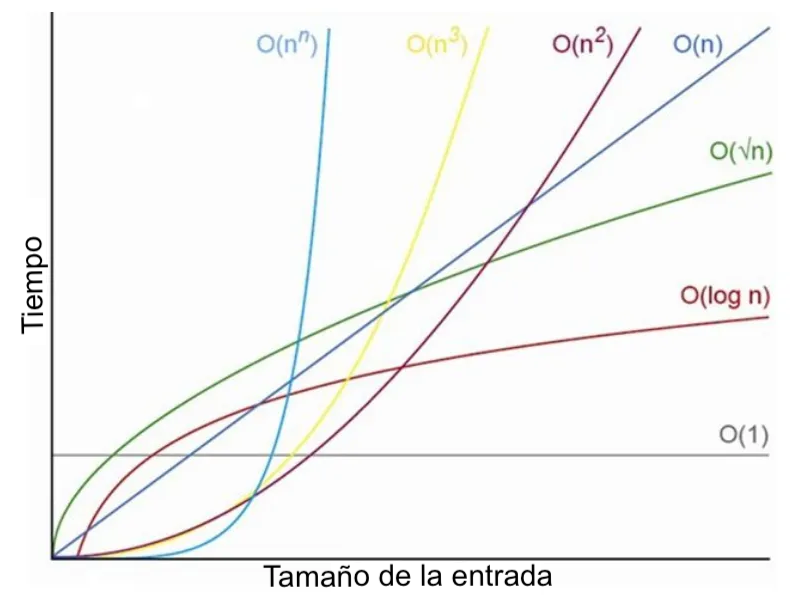
\includegraphics[width=200px]{./images/big_o_comparison.png}
  \caption{Big O - Comparación de complejidades}
  \label{fig:big_o_comparison}
\end{figure}

Diferentes implementaciones de un mismo algoritmo que resuelve un problema dado pueden tener diferentes complejidades,
Por ejemplo, para hay varios algoritmos que resuelven el problema de ordenar un \textit{array} (arreglo) de elementos de
tamaño $n$. El más popular por su facilidad de implementación es el algoritmo de
\href{https://es.wikipedia.org/wiki/Ordenamiento_de_burbuja}{burbujeo} que, si bien ordena los elementos, tiene una
complejidad de $O(n^2)$, pero si utilizamos un algoritmo de ordenamiento más eficiente, nos encontramos con el
\href{https://es.wikipedia.org/wiki/Ordenamiento_por_mezcla}{\textit{merge sort}} que tiene una complejidad de $O(n
\cdot \; \log \; n)$. Ambos algoritmos resuelven el mismo problema (ordernar un array), pero uno es mucho más eficiente
que el otro. A veces, descubrir un algoritmo más eficiente no es tan fácil.

\textbf{El n es la cantidad de elementos que tenemos como input de nuestro algoritmo}. Con lo cual, un algoritmo que
tiene una entrada de tamaño $n$ y se ejecuta con una cierta función de tiempo $f(n)$, diremos que el algoritmo se
comporta con una complejidad asintótica de $O(g(n))$ si existe una constante $C$ y un valor $n_0$ tal que el valor
absoluto de $f(n)$ es menor o igual a $C$ por el valor absoluto de $g(n)$ para todo $n$ mayor a $n_0$.
(\textcite{wilf2002}). Formalmente:

\[
  f(n) = O(g(n)) \; (x \; \rightarrow \; \infty) \; si \; \exists \; C, n_0 \; \slash \; \lvert f(n) \rvert \leq C \,
  \lvert g(n) \rvert \; (\forall \; n > n_0)
\]

Las diferentes complejidades algorítmicas deberán ser realizables; y por \textit{realizables} queremos decir que la
capacidad de resolver las instancias deseadas de un problema estén dentro de nuestros recursos disponibles. En la
práctica, la factibilidad es muy dependiente del contexto y no es particularmente \textit{portable} (portátil) entre
diferentes problemas y situaciones. Un principio común se mantiene en casi todas las situaciones: \textbf{una tasa de
crecimiento exponencial en el consumo de algún recurso limita la aplicación del uso de ese método a todas las
instancias, excepto a las más pequeñas}. En otras palabras, si nuestros algoritmos tienden a tener complejidades
exponenciales (o más) en el tamaño de la entrada, no importa cuántos recursos tengamos, no podremos resolver instancias
grandes del problema. Por lo tanto, la factibilidad ha llegado a significar que la tasa de crecimiento del recurso está
acotada por un una complejidad polinomial en el tamaño de la entrada. Esto nos da la noción común de que un problema
tiene una solución secuencial factible sólo si tenemos un algoritmo de tiempo polinomial, es decir, sólo si cualquier
instancia de tamaño $n$ del problema se puede resolver en tiempo $n^{O(1)}$. Aunque ampliamente reconocido como muy
simplista, la dicotomía entre algoritmos polinomiales y no polinomiales ha demostrado ser un discriminador poderoso
entre aquellos cálculos que son factibles en la práctica y aquellos que no lo son (\textcite{greenlaw1995}).

Lógicamente hay problemas para los cuales no se han encontrado algoritmos polinomiales, por ejemplo, la factorización
entera de un número muy grande es un problema que no puede resolverse en tiempo polinomial con las CPUs y GPUs actuales.
Por eso es que la seguridad de muchos sistemas de encriptación se basan en ello. Si bien excede lárgamente el contenido
de esta materia, hay algoritmos cuánticos que pueden resolver este problema en tiempo $O((\log n)^{O(1)})$
(\cite{ekert1996}).

\subsection*{¿Por qué no se utilizan GPUs para todo?}

En la \ref{sec:introduccion} se mencionó que el \textit{ratio} de rendimiento entre una CPU y una GPU puede ser de 1:10
(e incluso mayor), entonces una pregunta válida sería \textbf{¿por qué no se utilizan GPUs para todo?}. La respuesta a
esto no es única, por un lado las GPUs están diseñadas para tener alto \textit{throughput} de operaciones matemáticas y
de transferencia a memoria y suelen ser buenas para tareas de alta latencia que requieren pasajes grandes de información
desde y hacia la memoria (óptimos para el procesamiento paralelo). Por el otro lado las CPUs están optimizadas para
realizar tareas de baja latencia y tareas inherentemente secuenciales donde sorbepasan holgadamente a la
\textit{performance} de una GPU. Por esto es que estos sistemas se llaman híbridos, ya que hay un hilo conductor
secuencial y otros que se ejecutan en paralelo (a demanda).

\textbf{La parelelización es importante ya que hay aplicaciones que trabajan con datos que pueden ser procesados en
paralelo utilizando varias GPUs}. Por ejemplo en biología donde a veces las observaciones están limitadas por las
observaciones que se pueden hacer a nivel molecular con lo cual, creando modelos que simulen las actividades subyacentes
de estas moléculas a través de modelos computacionales se pueden hacer simulaciones que permitan hacer predicciones
sobre el comportamiento de estas moléculas.

Como veremos en la sección siguiente, no todas las aplicaciones pueden ser paralelizadas, y en muchas aplicaciones, sólo
un porcentage del tiempo de ejecución de una aplicación puede ser paralelizado, lo cual implica que es el algoritmo
utilizado quien define la mejora de velocidad, no necesariamente el número de procesadores; en algún momento llegaremos
a un límite donde finalmente por más que tengamos más recursos no se podrá paralelizar más el algoritmo. A esto se lo
conoce como \href{https://es.wikipedia.org/wiki/Ley_de_Amdahl}{ley de Amdahl}.

Al desarrollar CUDA C, NVIDIA no sólo ha permitido paralelizar aplicaicones, sino que también ha permitido bajar el
costo del desarrollo del software paralelo que estaba restringido a supercomputadoras masivamente paralelas. Esto se
debe a que el mercado actual de GPUs es enorme ya que casi todas las PCs actuales tienen algún tipo de GPU instalada,
habiendo más de 1000 millones de GPUs en el mundo que pueden ser utilizadas con CUDA, con lo cual al facilitar el
desarrollo de aplicaciones paralelas, NVIDIA logra hacer que el desarrollo de software paralelo sea más accesible para
todos.

\section*{Desafíos en la programación paralela}

Podríamos pensar entonces que la programación paralela puede ser una solución inherente para resolver todos los
problemas de rendimiento y debería utilizarse siempre. Aunque como vimos con la ley de Amdahl, no todos los problemas
son $100\%$ paralelizables, y en general sólo podremos intentar paralelizar una parte de la aplicación.

<<<<<<< Updated upstream
Sin embargo, por un lado es complicado diseñar algoritmos paralelos que tengan el mismo nivel de complejidad
computacional que los algoritmos secuenciales. Por el otro lado la programación paralela tiene límites de velocidad de
acceso a memoria. La performance de los algoritmos paralelos son muy sensibles a los datos de entrada, ya que
esencialmente la parelización se basa en el procesamiento de datos de manera paralela. Por último, pero no menos
importante, los algoritmos paralelos suelen expresarse de manera de recurrencias, lo cual requiere que se piensen los
diferentes problemas de formas no intuitivas.

||||||| Stash base
Sin embargo, por un lado es complicado diseñar algoritmos paralelos que tengan el mismo nivel de complejidad
computacional que los algoritmos secuenciales. Por el otro lado la programación paralela tiene límites de velocidad de
acceso a memoria. La performance de los algoritmos paralelos son muy sensibles a los datos de entrada, ya que
esencialmente la parelización se basa en el procesamiento de datos de manera paralela. Por último, pero no menos
importante, los algoritmos paralelos suelen expresarse de manera de recurrencias, lo cual requiere que se piensen los
diferentes problemas de formas no intuitivas.

Pero los problemas antes mencionados sólo son problemas técnicos que se podrían resolver con el tiempo y la suficiente
dedicación, pero podríamos preguntarnos si \textbf{¿todos los problemas son paralelizables?}.

\subsection*{Los límites de la programación paralela}

Una rama de la teoría de la complejidad computacional se dedica a identificar los problemas más difíciles en la clase P,
que son los problemas que pueden ser resueltos en tiempo polinomial. Estos problemas son de interés porque parecen
carecer de soluciones altamente paralelas. Es decir, los diseñadores de algoritmos han fallado en encontrar algoritmos
NC, soluciones paralelas altamente factibles que toman tiempo polinomial en el logaritmo del tamaño del problema
mientras usan sólo un número polinomial de procesadores. En consecuencia, la promesa de la computación paralela, es
decir, que aplicar más procesadores a un problema puede acelerar en gran medida su solución, parece ser rota por toda la
clase de problemas P-completo. Esto se puede escribir como $P = NC$.

En la teoría de complejidad computacional, P es una clase de complejidad que contiene todos los problemas de decisión
que pueden ser resueltos por una máquina de Turing determinista en tiempo polinomial. Sin embargo,
\href{https://en.wikipedia.org/wiki/Nick_Pippenger}{Nicholas Pippenger} realizó una investigación exhaustiva sobre
circuitos con profundidad polilogarítmica y tamaño polinomial y sugirió una interesante clase de complejidad a estudiar
que sería la clase de problemas solucionables por máquinas paralelas en tiempo polilogarítmico \footnote{Un problema es
polilogarítmico si su complejidad es $O((\log n)^k)$ para algún $k$} usando un número polinomial de procesadores. Esta
clase se conoce como \textbf{NC} (por \textit{Nick's class}). \cite{stockmeyer1987}

La clase P se puede pensar como los problemas tratables (tesis de Cobham), por lo que NC se puede pensar como los
problemas que se pueden resolver eficientemente en una computadora paralela. NC es un subconjunto de P porque los
cálculos paralelos polilogarítmicos se pueden simular mediante cálculos secuenciales polinomiales. Pero no se sabe si
NC = P, pero la mayoría de los investigadores sospechan que esto es falso, lo que significa que probablemente hay
algunos problemas tratables que son "intrínsecamente secuenciales" y no se pueden acelerar significativamente utilizando
paralelismo. Así como la clase NP-completo se puede pensar como "probablemente intratable", así que la clase P-completo,
cuando se utilizan reducciones NC, se puede pensar como "probablemente no paralelizable" o "probablemente
intrínsecamente secuencial".

\textbf{Con lo cual la respuesta a la pregunta de si todos los problemas son paralelizables es que NO}, hay ciertos
problemas que son intrínsecamente secuenciales y no se pueden paralelizar.

=======
El primer problema, es que es difícil diseñar algoritmos paralelos, ya que requiere pensar los problemas de formas
anti-intuitivas que, muchas veces, no son sencillas de resolver para que tengan el mismo nivel de complejidad
computacional que los algoritmos secuenciales. La performance de los algoritmos paralelos son muy sensibles a los datos
de entrada, ya que esencialmente la paralelización se basa en el procesamiento de datos de manera limitada por la
velocidad de acceso a memoria. Pero aún si salváramos estos problemas que son, méramente técnicos, nos encontraríamos
con la pregunta más profunda: \textbf{¿todos los problemas son teóricamente paralelizables?}.

\subsection*{Los límites de la programación paralela}

En la teoría de complejidad computacional, P es una clase \footnote{En matemáticas, una clase es una colección de
conjuntos (u otros objetos matemáticos) que pueden ser definidos unívocamente por una propiedad compartida por todos los
miembros de ese conjunto} de complejidad que contiene todos los problemas de decisión que pueden ser resueltos por una
máquina de Turing determinista en tiempo polinomial. Sin embargo,
\href{https://en.wikipedia.org/wiki/Nick_Pippenger}{Nicholas Pippenger} realizó una investigación exhaustiva sobre
circuitos con profundidad polilogarítmica y tamaño polinomial y sugirió una interesante clase de complejidad a estudiar
que sería la clase de problemas solucionables por máquinas paralelas en tiempo polilogarítmico \footnote{Un problema es
polilogarítmico si su complejidad es $O((\log n)^k)$ para algún $k$} usando un número polinomial de procesadores. Esta
clase se conoce como \textbf{NC} (por \textit{Nick's class}). (\textcite{stockmeyer1987})

Los problemas $P-completos$ son de interés porque parecen carecer de soluciones altamente paralelas. Es decir, los
diseñadores de algoritmos han fallado en encontrar algoritmos \textit{NC}. En consecuencia, la promesa de la computación
paralela, es decir, que aplicar más procesadores a un problema puede acelerar en gran medida su solución, parece estar
ser imposible en toda la clase de problemas $P-completos$. Dejando abierta la siguiente pregunta:
(\textcite{greenlaw1995})

\[
  P \stackrel{?}{=} NC
\]

Esta clase P se puede pensar como los problemas tratables (tesis de Cobham), por lo que \textit{NC} se puede pensar como
los problemas que se pueden resolver eficientemente en una computadora paralela. NC es un subconjunto de P porque los
cálculos paralelos polilogarítmicos se pueden simular mediante cálculos secuenciales polinomiales. Pero no se sabe si
$NC \stackrel{?}{=} P$, pero \textbf{la mayoría de los investigadores sospechan que esto es falso}, lo que significa que
probablemente hay algunos problemas tratables que son \textbf{"intrínsecamente secuenciales"} y no se pueden acelerar
significativamente utilizando paralelismo. Así como la clase NP-completo se puede pensar como "probablemente
intratable", así que \textbf{la clase P-completo, cuando se utilizan reducciones NC, se puede pensar como "probablemente
no paralelizable" o "probablemente \textit{intrínsecamente secuencial}"}.

Con lo cual, \textbf{la respuesta a la pregunta de si todos los problemas son paralelizables es que NO, ya que hay
ciertos problemas que son intrínsecamente secuenciales y no se pueden paralelizar}.

>>>>>>> Stashed changes
\section*{Modelos y Lenguajes de Programación Paralela}

En el pasado hubo muchos lenguajes de programación que fueron propuestos para abordar el problema de la programación
paralela. Algunos de estos lenguajes son:

\begin{itemize}
  \item \textbf{OpenMP}: es una API de programación en paralelo que se basa en directivas de compilador y funciones de
    biblioteca para permitir la paralelización de aplicaciones en sistemas de memoria compartida.
  \item \textbf{MPI}: es una biblioteca de paso de mensajes que permite la comunicación entre procesos en un sistema
    distribuido.
  \item \textbf{OpenACC}: Es un estándar de programación para la computación paralela desarrollado por Cray, CAPS,
    Nvidia y PGI. El estándar está diseñado para simplificar la programación paralela de sistemas heterogéneos CPU/GPU.
  \item \textbf{OpenCL}: Es un estándar abierto para la programación de sistemas heterogéneos que consta de CPUs, GPUs y
    otros dispositivos de cómputo.
  \item \textbf{CUDA}: Es una plataforma de computación paralela y un modelo de programación desarrollado por NVIDIA para
    sus GPUs.
\end{itemize}

\newpage

\vspace{1em}

\printbibliography


\end{document}
